\documentclass[../../main.tex]{subfiles}

\begin{document}
    Im nächsten Abschnitt befassen wir uns nun konkreter mit unserer Heimatgalaxie, der Milchstraße. Ziel ist zunächst die Validierung einer Annahme unserer späteren kartographischen Berechungen, welche die Konstanz der Bahngeschwindigkeit der um das galaktische Zentrum zirkulierenden wasserstoffhaltigen Wolken voraussetzt. 
    
    Hierzu betrachten wir den Sternenhimmel bezüglich des galaktischen Koordinatensystems bei $\SI{0}{\degree}$ galaktischer Breite und zwischen $\SI{30}{\degree}$ und $\SI{90}{\degree}$ galaktischer Länge, wobei wir die Abtastung mit Schrittweite $\delta l := \SI{5}{\degree}$ gemäß $s(t) := \delta l\cdot t + \SI{30}{\degree}$ durchführen. Durch unser Teleskop erhalten wir Intensitätswerte zu bereits umgerechneten relativen Geschwindigkeiten, aus welchen wir für jeden Raumwinkel den Maximalwert ermitteln. Hierzu verwenden wir eine Peak-Detektion mittels Gaußfunktionen
    \[
        G_{A,c,\sigma}(x) := A\cdot\exp(-\frac{(x-c)^2}{2\cdot\sigma^2}).
    \] 
    Die Amplitude $A\in\R$ ergibt sich aus der gemessenen Intensität, das Zentrum $c\in\R$ durch den Intensitätspeak, verursacht durch eine vermessenen Wolke. Für unser Ziel hat die Standardabweichung $\sigma\in\R$ keine Bedeutung. Eine Kurvenanpassung erfolgt nach Glättung des Datensatzes mittels Glättungskern $j$ und Faltung des Datensatzes $\mathcal{D}$ mit diesem, sowie Ermittelung lokaler Maxima im Intensitätsbereich $\R_{>5}$. Die Anzahl der maximierenden Elemente aus $\text{argmax}(j\ast\mathcal{D})$ gibt die Anzahl der nötigen Gaußfunktionen $G$ wieder, wobei wir für $x_0\in\text{argmax}(j\ast\mathcal{D})$ als Startwert $G(\mathcal{D}(x_0),x_0,5)$ raten und über die Argumentmenge summieren: $\mcG(x) := \sum_{x_0\in\text{argmax}(j\ast\mathcal{D})}G(\mathcal{D}(x_0),x_0,5)(x)$ ist damit unsere Anpassungsfunktion. Optisch analysieren wir einen Datensatz also wie in Abbildung \ref{fig:combined_spectrum_64939} dargestellt. 
    \begin{figure}[H]
        \centering
        \includegraphics[width=0.8\textwidth]{Bilddateien/MilkyVelocity/combined_spectrum_64939.pdf}
        \caption{Optische Darstellung der Peak-Detektion an einem gemessenen Spektrum bei $\SI{35}{\degree}$ galaktischer Länge.}
        \label{fig:combined_spectrum_64939}
    \end{figure} 
    Die hieraus erhaltenen Maximalwerte müssen wir nun zu einer Radialgeschwindigkeit von angenommenen Kreisbahnen um das galaktische Zentrum Saggittarius $\text{A}^*$ umrechnen. Hierzu bedienen wir uns folgender geometrischer Überlegung: Betrachten wir eine Wolke $M$ auf gerader Strecke $\overline{SM}$ von der Sonne $S$ aus (der Abstand Erde-Sonne ist aufgrund der galaktischen Längenskalen vernachlässigbar), so können wir über die Beziehung 
    \[
        R(l) := R_{\odot}\cdot\sin(l), \qquad R_{\odot} := \SI{8.5}{\kilo\parsec}
    \]
    den Abstand $R(l)$ der Wolke $M$ zum galaktischen Zentrum in Abhängigkeit der galaktischen Länge $l$ bestimmen. 
    % Mögliche weitere Erläuterung
    Für die gesuchte Tangentialgeschwindigkeit $V_t$ ergibt sich ferner
    \[
        V_t\bigl(V_{r,max},l\bigr) = V_{r,max} + V_{\odot}\cdot\sin(l), \qquad V_{\odot} := \SI{220}{\kilo\meter\per\second}.
    \] 
    Visuell unterstreicht Abbildung \ref{fig:GeometrieGalaxie} die skizzierten geometrischen Zusammenhänge.
    \begin{figure}[H]
        \centering
        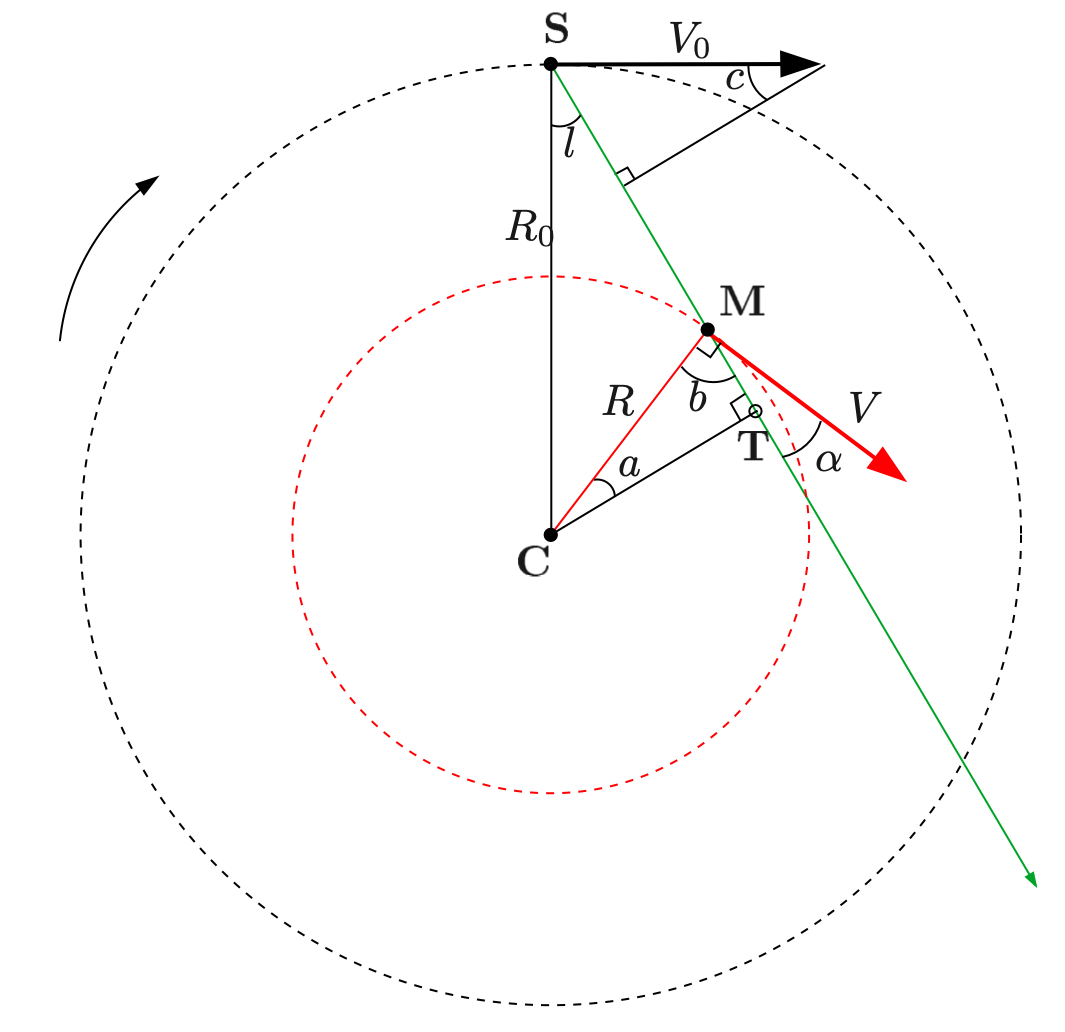
\includegraphics[width=0.6\textwidth]{Bilddateien/MilkyVelocity/GeometrieGalaxie.pdf}
        \caption{Darstellung der galaktischen Geometrie. Dabei steht S für den Standort der Sonne, C für das galaktische Zentrum und M für eine wasserstoffhaltige Wolke. Die Vektoren R und $\text{R}_0$ geben dabei entsprechende Abstände und V die Geschwindigkeit der Wolke an \cite[p.9]{doc:SALSAStudentManual}.}
        \label{fig:GeometrieGalaxie}
    \end{figure}
    In dieser zweiten Gleichung kommt nun der oben ermittelte Maximalwert $V_{r,max}$ zum Einsatz. Wir erhalten unter Berücksichtigung der geometrischen Zusammenhänge die in Abbildung \ref{fig:velocity_radius} dargestellte Abhängigkeit der Tangentialgeschwindigkeit vom Abstand zum galaktischen Zentrum.
    \begin{figure}[H]
        \centering
        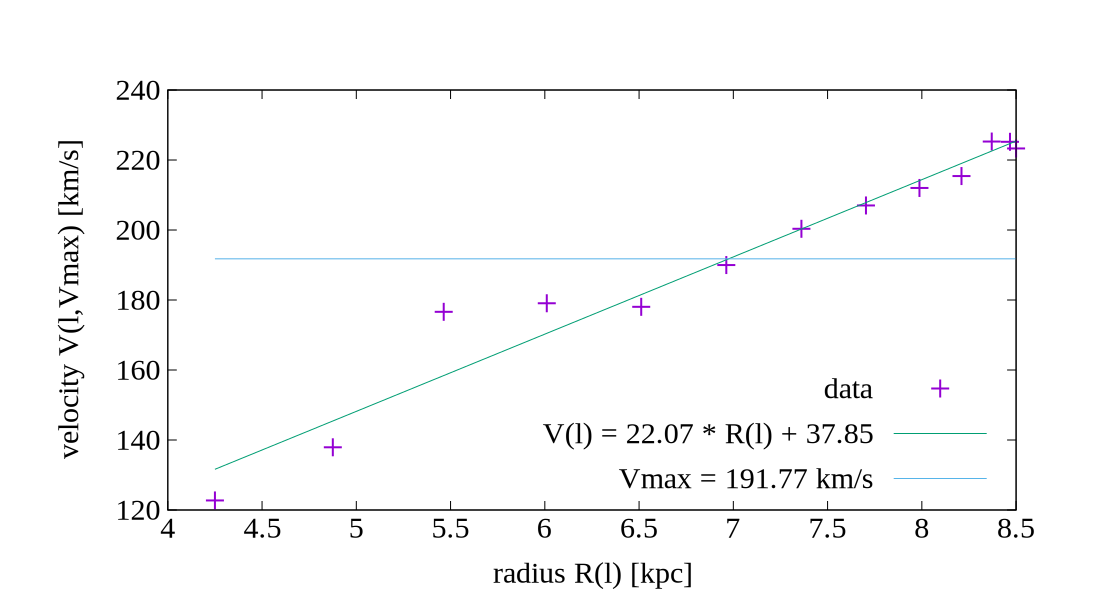
\includegraphics[width=0.8\textwidth]{Bilddateien/MilkyVelocity/velocity_radius.pdf}
        \caption{Relative Maximalgeschwindigkeit gemessener wasserstoffhaltiger Wolken in Abhängigkeit des Abstands zum galaktischen Zentrum.}
        \label{fig:velocity_radius}
    \end{figure}
    Klar ersichtlich ist zunächst eine hohe Schwankung der Werte um den kurvenangepassten Mittelwert $\langle V\rangle = \SI{213.33}{\km\per\s}$. Die Standardabweichung des Wertes beläuft sich hingegen auf $\SI{1.606}{\km\per\s}$, was $\SI{0.753}{\percent}$ des Wertes entspricht. Somit liegt die Sonnengeschwindigkeit $V_{\odot}$ zwar in der Nähe des Mittelwertes $\langle V\rangle$, jedoch nicht in dem ermittelten Unsicherheitsintervall $[V_\odot - 1.606,V_\odot + 1.606]$. Abhilfe schafft hier eventuell die unbekannte Unsicherheit der Datensätze, welche sich weiter durch die einzelnen Prozessschritte zur Ermittlung der Peaks durchziehen würde. Hierbei wäre insbesondere die Unsicherheitsfortpflanzung durch die vorgenommene Glättung mittels Faltung zu betrachten, sowie die Unsicherheit der Gaußfunktionen und die optisch bereits erkennbare Verschiebung ihrer Zentren gegenüber der tatsächlichen lokalen Maxima des Datensatzes, siehe hierzu Abbildung \ref{fig:combined_spectrum_64939}. Da wir hier nur eine qualitative Betrachtung durchgeführt haben, müssen wir auf eine weitere Verfeinerung der Unsicherheiten an dieser Stelle verzichten. 

    \subsubsection*{Genauere Unsicherheitsidee}
        Nehmen wir an, wir wollten die Unsicherheit ausgehend vom Datensatz $\mathcal{D}$ bestimmen und würden uns auf die Unsichereheitsfortpflanzung $u_{\textit{pf}}$ beschränken. Wir definieren hierzu den Operator $u_{\textit{pf}}$ für Funktionen $f\in C^1(\R^d,\R)$ als 
        \[
            u_{\textit{pf}}(f) := \fdef{
                \sqrt{
                    \sum_{i\in [d]}\partial_if(x)^2\cdot u(x)_i^2
                }
            }{x\in\R^d} = \fdef{\dabs{df(x)(u(x))}{2}}{x\in\R^d},
        \]
        wobei $u$ die Unsicherheit des Argumentes $x$ bezeichnet. Für den Datensatz $\mathcal{D}:\R\to\R$ gilt also $u_{\textit{pf}}(\mcD)(x) = \sqrt{\mathcal{D}'(x)^2\cdot u(x)^2}$. Sei $j$ ein Faltungskern, so ist gemäß Faltungsdefinition von integrierbaren Funktionen $f:\R\to\R$ die Faltung $(j\ast f)(x) = \int_{\R}j(x-y)f(y)dy$, also in Form eines Operators $\mathbb{J}(f)(x) := (j\ast f)(x)$. Um die Unsicherheit dieser Operation auf ähnliche Weise festzustellen, müssten wir einen Unsicherheitsoperator $\tilde u$ auf $\mathbb{J}$ in Auswertung $f$ anwenden:
        \[
            \tilde u(\mathbb{J})(f)(x) = \sqrt{\mathbb{J}'(f)(x)^2\cdot u_{pf}(f)(x)^2}.
        \]
        Ob der Ableitungstensor $\mathbb{J}'$ jedoch existiert, ist uns aufgrund $f\in (\R\to\R)$ aufgrund der unendlichen Dimensionalität nicht klar. An dieser Stelle wären weitere Überlegungen dringend empfohlen. 

\end{document}